\chapter{T\'{\i}tulo del primer cap\'{\i}tulo}\label{chap:fundamentos}

Each of your chapters will require both an introduction and a conclusion. The former
provides the reader with a contents `map' of what is to come, and the latter provides a
concise summary of what they have just read. 

\section{Primera Secci\'on}
Each introduction should look back to
the conclusion of the previous chapter, and forwards to the contents of the chapter
which you are introducing. The conclusion should look back into the chapter just
completed, and forward to the introduction of the following chapter. These
conclusions and introductions act like small links which bind the `chain' of the
chapters together in a more seamless whole than would have occurred if the chapters
had not been introduced or concluded; they `smooth out'  the transition from chapter
to chapter and from topic to topic. (Tomado de \cite{guidedissertation}.)


\subsection{Primera sub-secci\'on de la Primera Secci\'on}
\label{subsec:unaparaempezar}
Algo de texto y una gr\'afica para ver esta primera subsecci\'on.
\begin{figure}
  \begin{center}
   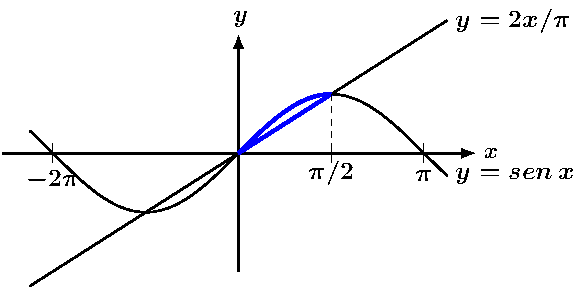
\includegraphics[scale=0.8]{./ilustraciones/fig1.pdf}
   \end{center}
   \caption{Una gr\'afica siempre viene bien para ilustrar el texto.}
   \label{fig:ejemplografica}
\end{figure}

No siempre aparecen las figuras (y las tablas) en el lugar exacto donde se
ponen en el archivo .tex. Aunque se tiene un cierto control sobre ello con los par\'ametros, al final es \LaTeX{} quien decide d\'onde ponerla.

Tambi\'en puede ser \'util poner tablas.
\begin{table}
\begin{center}
   \begin{tabular}{ r @{\hspace{1.3em}} r @{\hspace{1em}} r r }
       \textbf{A\;} & \textbf{B\;} & \textbf{C\;} & \textbf{Resto} \\
       \hline\noalign{\smallskip} 
       44.2 & 5.1 & 6.1 & 2.3\\
       712.2 & 8.3 & 99.2 & 3.1\\
       \hline
   \end{tabular}
   \caption{\label{tab:pocoutil}
   Una tabla peque\~na pero in\'util. Bueno, al menos es peque\~na, \textquestiondown no?}
\end{center}
\end{table}

Puedo referirme m\'as tarde tanto a la figura~\ref{fig:ejemplografica} de la p\'agina~\pageref{fig:ejemplografica}
como a la tabla~\ref{tab:pocoutil} de la p\'agina~\pageref{tab:pocoutil}, ambas
de la la subsecci\'on~\ref{subsec:unaparaempezar}. Para ello utilizamos los
comandos \verb$\label$ \verb$\ref$ y \verb$\pageref$



\section{Segunda Secci\'on}
Primero definimos lo que es un \emph{matem\'atico}, ese ser rarito y ensimismado.
\begin{definition}[Paul Erd\H os]
  Un \emph{matem\'atico} es un dispositivo que convierte caf\'e en teoremas.
\end{definition}
\begin{conjecture}
Me parece que se me va a olvidar todo esto.
\end{conjecture}
\begin{corollary}
Para qu\'e me lo voy a aprender.
\end{corollary}

\subsection{Primera sub-secci\'on de la Segunda Secci\'on}

\subsubsection{Primera sub-sub-secci\'on de la Primera subsecci\'on de la Segunda Secci\'on}
\begin{itemize}
  \item primer elemento de la lista
  \item este es el segundo
  \item y hay un tercero que se divide
  \begin{itemize}
    \item primera subdivisi\'on
    \item segundo tipo del tercer elemento
  \end{itemize}
\end{itemize}

Conviene tener en cuenta que al combinar los distintos atributos en las fuentes
de texto, no siempre resulta lo esperado:
\begin{center}
\begin{tabular}{cccccc}
      &    &\small\verb;\upshape; & \small\verb;\itshape;
           &\small\verb;\slshape; & \small\verb;\scshape;\\
\cline{2-6}
\small\verb;\rmfamily; & \small\verb;md; &
  \rmfamily\mdseries\textup{vertical} &
  \rmfamily\mdseries\textit{it\'alica}&
  \rmfamily\mdseries\textsl{inclinada}&
  \rmfamily\mdseries\textsc{Versalita}\\
      & \small\verb;bf; &
  \rmfamily\bfseries\textup{vertical} &
  \rmfamily\bfseries\textit{it\'alica}&
  \rmfamily\bfseries\textsl{inclinada}&
  \rmfamily\bfseries\textsc{Versalita}\\
\cline{2-6}
\small\verb;\sffamily; & \small\verb;md; &
  \sffamily\mdseries\textup{vertical} &
  \sffamily\mdseries\textit{it\'alica}&
  \sffamily\mdseries\textsl{inclinada}&
  \sffamily\mdseries\textsc{Versalita}\\
      & \small\verb;bf; &
  \sffamily\bfseries\textup{vertical} &
  \sffamily\bfseries\textit{it\'alica}&
  \sffamily\bfseries\textsl{inclinada}&
  \sffamily\bfseries\textsc{Versalita}\\
\cline{2-6}
\small\verb;\ttfamily; & \small\verb;md; &
  \ttfamily\mdseries\textup{vertical} &
  \ttfamily\mdseries\textit{it\'alica}&
  \ttfamily\mdseries\textsl{inclinada}&
  \ttfamily\mdseries\textsc{Versalita}\\
      & \small\verb;bf; &
  \ttfamily\bfseries\textup{vertical} &
  \ttfamily\bfseries\textit{it\'alica}&
  \ttfamily\bfseries\textsl{inclinada}&
  \ttfamily\bfseries\textsc{Versalita}\\
\cline{2-6}
\end{tabular}
\end{center}

